\documentclass{standalone}
\usepackage{tikz} % Import the tikz package
\usetikzlibrary{automata} % Import library for drawing automata
\usetikzlibrary{positioning} % ...positioning nodes
\usetikzlibrary{arrows} % ...customizing arrows
\tikzset{node distance=2.5cm,
    every state/.style={
        align=center,
        semithick,
        fill=gray!10},
    initial text={},
    double distance=2pt,
    every edge/.style={
        draw,
        ->,>=stealth',
        auto,
        semithick}}
\let\epsilon\varepsilon
\begin{document}
    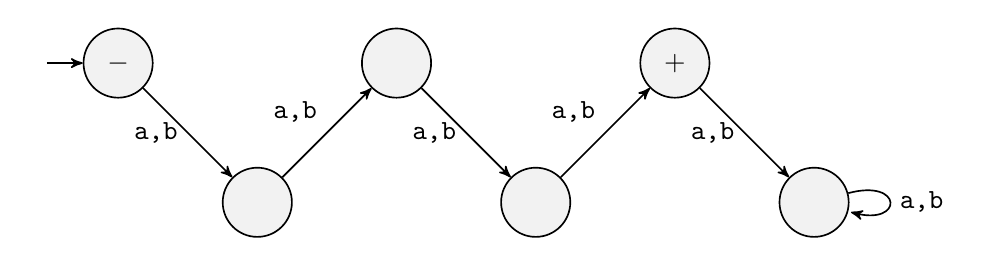
\begin{tikzpicture}
        \node[state,initial] (q1) {$-$};
        \node[state, below right of=q1] (q2) {};
        \node[state, above right of=q2] (q3) {};
        \node[state, below right of=q3] (q4) {};
        \node[state, above right of=q4] (q5) {$+$};
        \node[state, below right of=q5] (q6) {};

        \draw (q1) edge[left] node {\tt a,b} (q2);
        \draw (q2) edge node {\tt a,b} (q3);
        \draw (q3) edge[left] node {\tt a,b} (q4);
        \draw (q4) edge node {\tt a,b} (q5);
        \draw (q5) edge[left] node {\tt a,b} (q6);
        \draw (q6) edge[loop right] node {\tt a,b} (q6);
    \end{tikzpicture}
\end{document}